\documentclass[10pt,aspectratio=169]{beamer}

% Theme
\usetheme{Madrid}
\usecolortheme{beaver}

% Color scheme
\definecolor{darkblue}{RGB}{0,51,102}
\definecolor{accentred}{RGB}{180,30,30}
\definecolor{lightgray}{RGB}{240,240,240}
\setbeamercolor{frametitle}{fg=white,bg=darkblue}
%\setbeamercolor{title}{fg=white}
\setbeamercolor{author}{fg=white}
\setbeamercolor{institute}{fg=white}
\setbeamercolor{date}{fg=white}
%\setbeamercolor{structure}{fg=darkblue}
%\setbeamercolor{block title}{fg=white,bg=darkblue!75}
%\setbeamercolor{block body}{bg=darkblue!8,fg=black}
\setbeamercolor{alerted text}{fg=accentred}
\setbeamercolor{block title alerted}{fg=white,bg=accentred!85}
\setbeamercolor{block body alerted}{bg=accentred!8,fg=black}
\setbeamercolor{block title example}{fg=white,bg=darkblue!60}
\setbeamercolor{block body example}{bg=darkblue!5,fg=black}

% Packages
\usepackage[utf8]{inputenc}
\usepackage[T1]{fontenc}
\usepackage{amsmath,amssymb,amsfonts}
\usepackage{booktabs}
\usepackage{graphicx}
\usepackage{tikz}
\usepackage{pgfplots}
\pgfplotsset{compat=1.18}
\usepackage{multirow}
\usepackage{array}
\usepackage{hyperref}

% Settings
\setbeamertemplate{navigation symbols}{}
\setbeamertemplate{blocks}[rounded][shadow=true]
\setbeamertemplate{itemize items}[circle]
\setbeamertemplate{enumerate items}[default]

% Title
\title[Power Laws and Dengue]{Power Laws and Prediction Gaps:\\A Statistical Framework for Extreme Dengue Outbreaks in Brazilian Cities}
\author{Flavio Codeço Coelho}
\institute{Fundação Getulio Vargas (FGV) \\ Mosqlimate Researcch Group}
\date{April 2026}
\pgfdeclareimage[height=0.85cm]{mosq-logo}{mosqlimate_logo.png}
\pgfdeclareimage[height=0.95cm]{emap-logo}{Logo_FGV_EMAp}
\logo{
	\pgfuseimage{mosq-logo}
	\pgfuseimage{emap-logo}\hspace*{0.1cm}
	}

\begin{document}

% ============================================================
% SLIDE 1: Title
% ============================================================
{
\setbeamercolor{background canvas}{bg=darkblue}
\begin{frame}
\maketitle
\end{frame}
}

% ============================================================
% SLIDE 2: The Challenge of Dengue in Brazil
% ============================================================
\begin{frame}{The Challenge of Dengue in Brazil}
\begin{block}{The Problem}
\begin{itemize}
    \item \textbf{5,570 municipalities} across Brazil experience recurrent seasonal outbreaks
    \item Over \textbf{6 million reported cases} in a single epidemic season (2010--2012 pivotal study)
    \item Outbreak intensity varies by orders of magnitude: from tens to tens of thousands of cases per city per week
    \item Traditional surveillance models focus on \textbf{average transmission dynamics}, missing the risk of extreme events
\end{itemize}
\end{block}

\vspace{0.3cm}

\begin{block}{Public Health Impact}
\begin{itemize}
    \item Healthcare systems overwhelmed during peak outbreaks
    \item Resource allocation based on average predictions fails when extreme events occur
    \item \textbf{Critical gap:} no framework quantifies the probability of extreme outbreak magnitudes across heterogeneous geographic landscapes
\end{itemize}
\end{block}
\end{frame}

\begin{frame}{Underestimation}
	\centering
	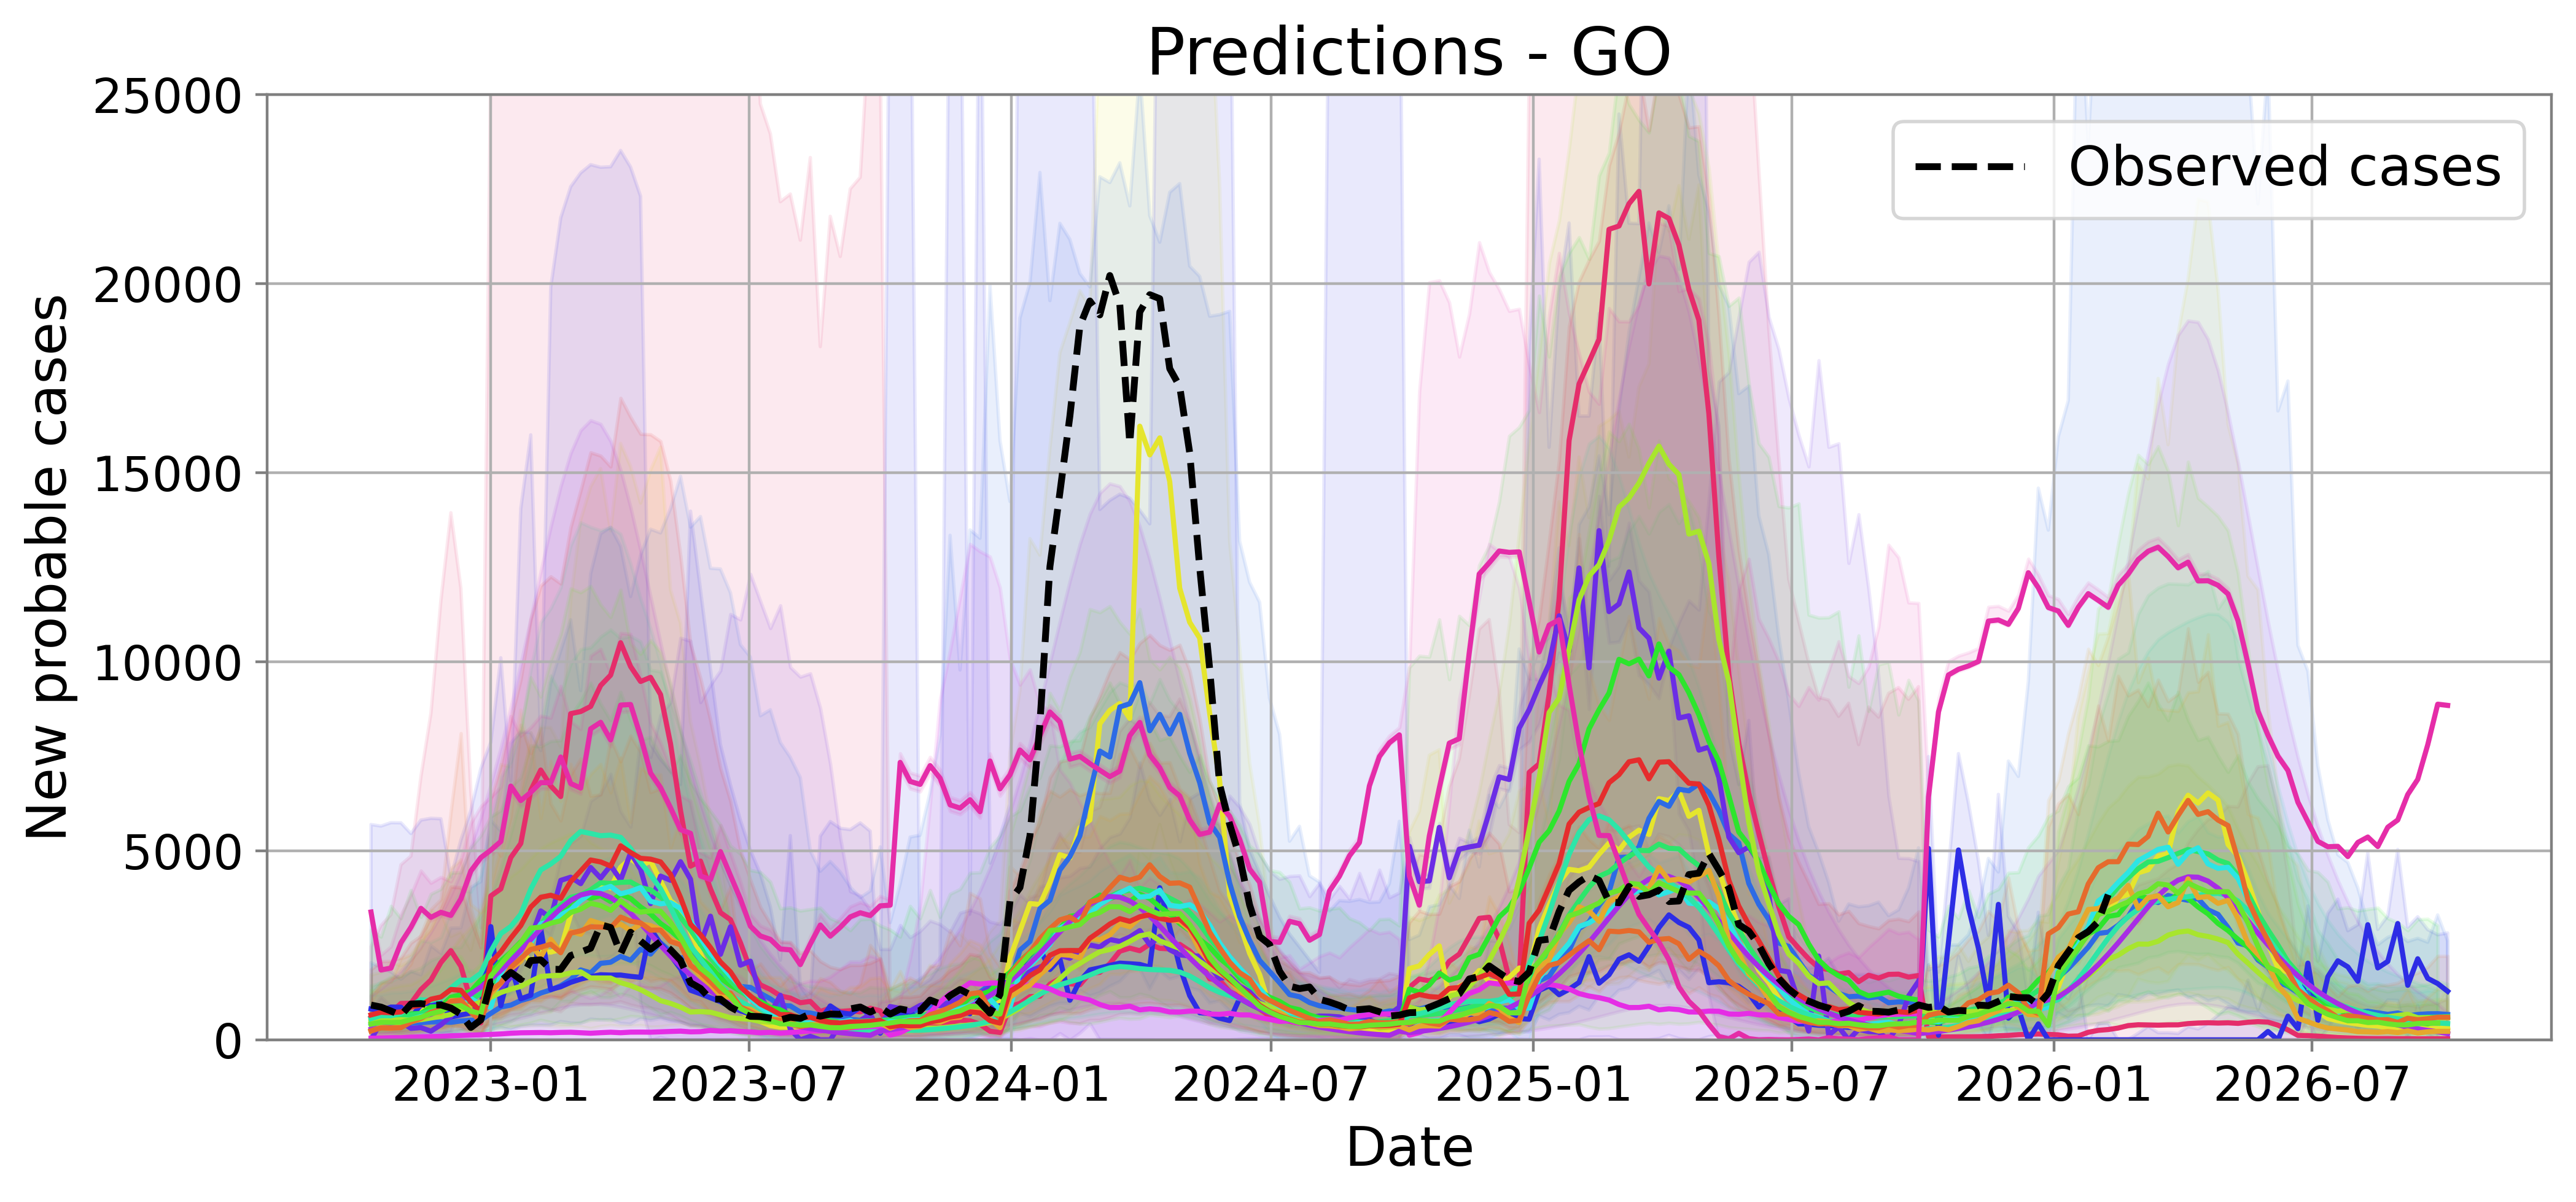
\includegraphics[width=\linewidth]{preds_GO.png} % ajuste largura

\end{frame}

% ============================================================
% SLIDE 3: Why Power Laws?
% ============================================================
\begin{frame}{Why Power Laws in Epidemiology?}
\begin{block}{Heavy-Tailed Distributions}
\begin{itemize}
    \item In a power law, the probability of extreme events decays as $P(X \geq x) \propto x^{-(\alpha-1)}$
    \item Unlike Normal distributions, \textbf{extreme events are far more likely} than Gaussian models predict
    \item The scaling exponent $\alpha$ encodes information about the underlying transmission dynamics
\end{itemize}
\end{block}

\vspace{0.3cm}

\begin{block}{Current Evidence}
\begin{itemize}
    \item \textbf{Rhodes et al. (1997):} Measles, pertussis, mumps in Faroe Islands follow power laws with $\tau \approx 2.1$--$2.4$
    \item \textbf{Dengue in Brazil:} Annual case counts follow power law with $\alpha = 2.06$ (constant over 12 years)
\end{itemize}
\end{block}
\end{frame}

% ============================================================
% SLIDE 4: Power Law — Mathematical Framework
% ============================================================
\begin{frame}{Power Law Distribution: Mathematical Framework}
\begin{block}{Definition}
A random variable $X$ follows a power law if its probability density function is:
$$p(x) = C \, x^{-\alpha}, \quad x \geq x_{\min}$$
where the normalization constant is:
$$C = (\alpha - 1)\, x_{\min}^{\,\alpha-1}$$
\end{block}

\vspace{0.2cm}

\begin{block}{Complementary CDF}
$$P(X \geq x) = \left(\frac{x}{x_{\min}}\right)^{-(\alpha-1)}$$
\begin{itemize}
    \item \textbf{$\alpha$ (scaling exponent):} Controls tail thickness. Lower $\alpha$ $\Rightarrow$ heavier tail $\Rightarrow$ more extreme events
    \item \textbf{$x_{\min}$ (lower bound):} Defines the onset of the scaling regime
    \item For discrete data: $p(x) = x^{-\alpha} / \zeta(\alpha, x_{\min})$ (Hurwitz zeta normalization)
\end{itemize}
\end{block}
\end{frame}

% ============================================================
% SLIDE 5: Power Laws in Epidemics — Literature
% ============================================================
\begin{frame}{Power Laws in Epidemics: Key Literature}
\begin{columns}[T]
\begin{column}{0.48\textwidth}
\textbf{Rhodes, Jensen \& Anderson (1997)}
\begin{itemize}
    \item Forest-fire model with sparks as analogy for Type III epidemics
    \item Scaling exponent $\tau$ correlates with $R_0$ (transmissibility)
    \item Conventional SEIR models fail to reproduce power law distributions
\end{itemize}

\vspace{0.3cm}

\textbf{Clauset, Shalizi \& Newman (2009)}
\begin{itemize}
    \item Gold-standard framework: MLE + KS test + likelihood ratio
    \item Log-log regression produces \textbf{biased} exponent estimates
    \item Many claimed power laws are better fit by log-normal
\end{itemize}
\end{column}

\begin{column}{0.48\textwidth}
\textbf{Komarova et al. (2020)}
\begin{itemize}
    \item Universal pattern: exponential $\to$ power law growth
    \item $\sim$70\% of countries show power law dynamics
    \item Metapopulation model: spatial spread generates power law from local exponential growth
\end{itemize}

\vspace{0.3cm}

\textbf{Li et al. (2012)}
\begin{itemize}
    \item Log Gaussian Cox Processes for spatial disease incidence
    \item Long-range spatial correlation with exponential cutoff
\end{itemize}
\end{column}
\end{columns}
\end{frame}

% ============================================================
% SLIDE 6: Estimation Methodology
% ============================================================
\begin{frame}{Estimation Methodology}
\begin{block}{The Clauset et al. (2009) Three-Step Recipe}
\begin{enumerate}
    \item \textbf{Parameter Estimation (MLE):}
    $$\hat{\alpha} = 1 + n \left[\sum_{i=1}^{n} \ln\left(\frac{x_i}{x_{\min}}\right)\right]^{-1}$$
    For discrete data, solve transcendental equation with Hurwitz zeta function.

    \vspace{0.2cm}

    \item \textbf{Goodness-of-Fit Test:}
    Compute KS statistic between empirical and fitted CDF. Generate bootstrap samples from fitted power law. $p > 0.1$ indicates power law is plausible.

    \vspace{0.2cm}

    \item \textbf{Comparison with Alternatives:}
    Likelihood ratio test (Vuong's method) against log-normal, exponential, stretched exponential, and power law with exponential cutoff.
\end{enumerate}
\end{block}

\begin{alertblock}{Key Requirement}
Minimum sample size: $n \gtrsim 50$ for reasonable estimates, $n \gtrsim 1000$ in the tail for robust testing.
\end{alertblock}
\end{frame}

% ============================================================
% SLIDE 7: Data & Computational Framework
% ============================================================
\begin{frame}{Data \& Computational Framework}
\begin{columns}[T]
\begin{column}{0.5\textwidth}
\textbf{Data Sources}
\begin{itemize}
    \item \textbf{Infodengue API:} Weekly dengue case counts (2010--2025) for all 5,570 Brazilian municipalities
    \item \textbf{Episcanner:} Epidemic-level metrics (size, duration, peak week, $R_0$, onset, residuals)
    \item \textbf{Mosqlimate API:} Climate covariates (temperature, humidity) at quarterly resolution
    \item \textbf{Demographics:} Municipal population and socioeconomic indicators
\end{itemize}

\vspace{0.3cm}

%\textbf{Data Pipeline}
%\begin{itemize}
%    \item Asynchronous data fetching with \texttt{asyncio}
%    \item \texttt{DuckDB} for efficient aggregation
%    \item \texttt{SQLite} database for fit results
%\end{itemize}
\end{column}

\begin{column}{0.45\textwidth}
%\textbf{Analysis Pipeline}
%\begin{itemize}
%    \item Power law fitting via \texttt{powerlaw} Python library
%    \item Spatial analysis with \texttt{PyGeoDa} (Local Moran's I)
%    \item Predictive modeling: \texttt{scikit-learn} Random Forest + LightGBM + HistGradientBoosting
%    \item Interactive Gradio dashboard for real-time exploration
%\end{itemize}

\vspace{0.3cm}
\begin{center}
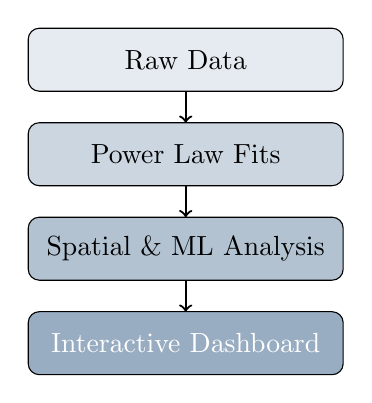
\begin{tikzpicture}
\node[draw, rectangle, rounded corners, fill=darkblue!10, minimum width=4cm, minimum height=0.8cm] {Raw Data};
\node[draw, rectangle, rounded corners, fill=darkblue!20, minimum width=4cm, minimum height=0.8cm] at (0,-1.2) {Power Law Fits};
\node[draw, rectangle, rounded corners, fill=darkblue!30, minimum width=4cm, minimum height=0.8cm] at (0,-2.4) {Spatial \& ML Analysis};
\node[draw, rectangle, rounded corners, fill=darkblue!40, text=white, minimum width=4cm, minimum height=0.8cm] at (0,-3.6) {Interactive Dashboard};
\draw[->, thick] (0,-0.4) -- (0,-0.8);
\draw[->, thick] (0,-1.6) -- (0,-2.0);
\draw[->, thick] (0,-2.8) -- (0,-3.2);
\end{tikzpicture}
\end{center}
\end{column}
\end{columns}
\end{frame}

% ============================================================
% SLIDE 8: Four-Pronged Analysis
% ============================================================
\begin{frame}{Four-Pronged Analytical Approach}
\begin{enumerate}
    \item \textbf{Longitudinal $\alpha$ Tracking}
    \begin{itemize}
        \item Yearly power law fitting for each city over 15 years
        \item OLS regression on $\alpha$ trends to detect regime shifts
        \item Identifies cities transitioning from predictable to extreme outbreak patterns
    \end{itemize}

    \vspace{0.15cm}
    \item \textbf{Spatial Clustering (Local Moran's I)}
    \begin{itemize}
        \item LISA analysis to identify hotspots of high/low $\alpha$ values
        \item Detects geographic clusters of extreme outbreak propensity
        \item Reveals spatial autocorrelation in scaling behavior
    \end{itemize}

    \vspace{0.15cm}
    \item \textbf{Epidemiological Correlations}
    \begin{itemize}
        \item $\alpha$ vs $R_0$, total cases, epidemic duration, onset timing, model residuals
        \item Links statistical scaling to mechanistic epidemic drivers
    \end{itemize}

    \vspace{0.15cm}
    \item \textbf{Predictive Modeling}
    \begin{itemize}
        \item Random Forest, LightGBM (quantile), HistGradientBoosting (quantile)
        \item Features: lagged metrics, $\alpha_{t-1}$, $x_{\min}$, $\dot{\alpha}$, $R_0$, $\log_{10}(\text{Pop})$, climate
        \item Targets: epidemic size $S_t$, duration $D_t$, peak week $P_t$
    \end{itemize}
\end{enumerate}
\end{frame}

% ============================================================
% SLIDE 9: Spatial Distribution of α
% ============================================================
\begin{frame}{Results: Spatial Distribution of $\alpha$}
\begin{block}{Geographic Heterogeneity}
\begin{itemize}
    \item \textbf{Significant spatial variation} in scaling exponent across Brazilian states and municipalities
    \item States with \textbf{low $\alpha$} (heavy tails): frequent extreme outbreaks, higher unpredictability?
    \item States with \textbf{high $\alpha$} (thin tails): more predictable epidemic dynamics, fewer extreme events?
\end{itemize}
\end{block}

\vspace{0.3cm}

\begin{block}{Interpretation of $\alpha$}
\begin{itemize}
    \item Lower $\alpha$ $\leftrightarrow$ thicker tail $\leftrightarrow$ higher probability of extreme outbreaks
    \item Analogous to Rhodes et al.'s finding that less transmissible diseases have \textbf{larger} $\tau$ (thinner tails)
    \item For dengue: $\alpha$ varies geographically, reflecting heterogeneity in transmission drivers (climate, demographics, immunity)
\end{itemize}
\end{block}

\begin{alertblock}{Key Insight}
The spatial map of $\alpha$ serves as a \textbf{risk atlas}: regions with heavy-tailed dynamics require disproportionate preparedness capacity relative to their average case burden.
\end{alertblock}
\end{frame}

% ============================================================
% SLIDE 10: Alpha Trends Over Time
% ============================================================
\begin{frame}{Results: Temporal Evolution of $\alpha$}
\begin{block}{Longitudinal Scaling Trends}
\begin{itemize}
    \item Yearly $\alpha$ estimates reveal \textbf{temporal trajectories} of epidemic dynamics
    \item Some cities show \textbf{stable $\alpha$}: consistent power law behavior over 15 years
    \item Others exhibit \textbf{regime shifts}: trending toward heavier or thinner tails
\end{itemize}
\end{block}

\vspace{0.3cm}

\begin{block}{Trend Analysis}
\begin{itemize}
    \item OLS slope of $\alpha$ over time: $\dot{\alpha} = \frac{d\alpha}{dt}$
    \item $\dot{\alpha} < 0$: city becoming more prone to extreme outbreaks
    \item $\dot{\alpha} > 0$: city becoming more predictable (thinner tails)
    \item $\dot{\alpha}$ used as a predictive feature in the ML model
\end{itemize}
\end{block}

\begin{exampleblock}{Connection to Komarova et al. (2020)}
Temporal shifts in $\alpha$ may reflect the universal transition from exponential to power law growth as epidemics mature across spatially distributed populations.
\end{exampleblock}
\end{frame}

% ============================================================
% SLIDE 11: Epidemiological Correlations
% ============================================================
\begin{frame}{Results: Epidemiological Correlations}
\begin{columns}[T]
\begin{column}{0.5\textwidth}
\textbf{Correlations with $\alpha$:}
\begin{itemize}
    \item \textbf{$R_0$:} Basic reproduction number linked to tail thickness --- higher transmission intensity associated with heavier tails
    \item \textbf{Total Cases:} $\alpha$ inversely related to attack rates --- cities with lower $\alpha$ experience larger cumulative outbreaks
    \item \textbf{Epidemic Duration:} Heavy-tailed case distributions correlate with longer outbreak seasons
    \item \textbf{Onset Timing:} Earlier epidemic onset associated with different scaling regimes
\end{itemize}
\end{column}

\begin{column}{0.45\textwidth}
\textbf{Model Residuals:}
\begin{itemize}
    \item Sum of residuals from epidemic curve fitting vs $\alpha$
    \item Cities with heavier tails show \textbf{larger residuals} in standard epidemic models
    \item This is the ``\textbf{prediction gap}'': conventional models systematically underperform in heavy-tailed regimes
\end{itemize}
\end{column}
\end{columns}

\vspace{0.3cm}

\begin{block}{Implication}
The scaling parameter $\alpha$ is not merely a statistical artifact --- it is an \textbf{emergent property} of the transmission system that encodes information about demography, climate, and epidemic dynamics.
\end{block}
\end{frame}

% ============================================================
% SLIDE 12: Epidemic Metrics Power Laws
% ============================================================
\begin{frame}{Results: Epidemic Metrics Power Laws}
\begin{block}{Extended Power Law Analysis}
Beyond weekly case counts, power laws also emerge in \textbf{epidemic-level metrics}:
\begin{itemize}
    \item \textbf{Epidemic Size} (total cases per outbreak): heavy-tailed distribution confirmed via MLE + KS tests
    \item \textbf{Epidemic Duration} (weeks): also exhibits scaling behavior, though with different exponents
\end{itemize}
\end{block}

\vspace{0.3cm}

\begin{block}{Combined CCDF Analysis}
\begin{itemize}
    \item Multi-year cumulative distribution functions with year-stratified visualization
    \item Yearly $\alpha$ trends overlaid on boxplots of metric distributions
    \item State-level aggregation reveals consistent patterns across aggregation levels
\end{itemize}
\end{block}

\begin{alertblock}{Consistency}
Power law scaling in weekly incidence and
epidemic size confirms that extreme outbreak dynamics are not limited to case counts --- they are a \textbf{structural property} of the epidemic system.
\end{alertblock}
\end{frame}

% ============================================================
% SLIDE 13: Predictive Modeling
% ============================================================
\begin{frame}{Results: Predictive Modeling}
\begin{columns}[T]
\begin{column}{0.5\textwidth}
\textbf{Model Architecture}
\begin{itemize}
    \item Predict year $t$ from year $t-1$ features
    \item \textbf{Models:}
    \begin{itemize}
        \item Random Forest (baseline)
        \item LightGBM (quantile loss)
        \item HistGradientBoosting (quantile loss)
    \end{itemize}
    \item \textbf{Targets:} $S_t$, $D_t$, $P_t$
    \item \textbf{Evaluation:} MAE, RMSE, Pinball Loss (quantile models), OOB R$^2$
\end{itemize}
\end{column}

\begin{column}{0.45\textwidth}
\textbf{Key Results}
\begin{itemize}
    \item Predicted vs Actual (log-log scale) shows good agreement across orders of magnitude
    \item Feature importance: lagged metrics + $\alpha$ features rank highly
    \item Quantile models (LightGBM, HGB) provide uncertainty bounds
    \item Population filter: removing small cities improves model performance
\end{itemize}
\end{column}
\end{columns}

\vspace{0.3cm}

\begin{block}{Residual Analysis}
\begin{itemize}
    \item Residuals vs Predicted: no systematic bias across prediction range
    \item Residual distributions approximately centered at zero
    \item Cities with $>$20\% error analyzed by population distribution
\end{itemize}
\end{block}
\end{frame}

% ============================================================
% SLIDE 13b: Size Classification Model
% ============================================================
\begin{frame}{Results: Size Classification Model --- Predicting Large Epidemics}
\begin{block}{Objective}
\begin{itemize}
    \item Binary classification: will city $i$ in year $t$ exceed the $p$-th percentile of historical case counts?
    \item Target: $Y_{i,t} = \mathbb{I}\big(S_{i,t} > \text{percentile}_{p}(S_{\text{train}})\big)$, where the threshold is computed \textbf{only on training folds} to prevent leakage
    \item Default: $p = 75$-th percentile (configurable: 50--99)
\end{itemize}
\end{block}

\vspace{0.2cm}

\begin{columns}[T]
\begin{column}{0.48\textwidth}
\textbf{Methodology}
\begin{itemize}
    \item \textbf{Models:} XGBoost, LightGBM classifiers
    \item \textbf{Validation:} TimeSeriesSplit (no shuffle) --- preserves temporal ordering
    \item \textbf{Imbalance:} \texttt{scale\_pos\_weight} (XGBoost), \texttt{is\_unbalance=True} (LightGBM)
    \item \textbf{Threshold optimization:} Youden's $J = \text{Sensitivity} + \text{Specificity} - 1$ on CV out-of-fold predictions
    \item \textbf{Interpretability:} Feature importance + SHAP values
\end{itemize}
\end{column}

\begin{column}{0.48\textwidth}
\textbf{Features ($X_{t-1}$)}
\begin{itemize}
    \item Lagged epidemic metrics: $S_{t-1}, D_{t-1}, P_{t-1}$
    \item Power law scaling: $\alpha_{t-1}, x_{\min, t-1}$
    \item Historical trend: $\dot{\alpha}_{t-1}$
    \item Epidemiological driver: $R_{0, t-1}$
    \item Demographics: $\log_{10}(\text{Pop})$
    \item Climate (quarterly): $\bar{T}_{Q1\ldots Q4}, \bar{H}_{Q1\ldots Q4}$
\end{itemize}
\end{column}
\end{columns}

\vspace{0.2cm}

\begin{block}{Evaluation Metrics}
AUC-ROC, AUC-PR, F1-Score, Precision, Recall, Brier Score, Calibration Curve, Confusion Matrix
\end{block}
\end{frame}

% ============================================================
% SLIDE 14: Key Findings
% ============================================================
\begin{frame}{Key Findings and Implications}
\begin{block}{Main Results}
\begin{enumerate}
    \item \textbf{Power law scaling is pervasive} in dengue incidence across Brazilian municipalities --- both in weekly case counts and epidemic-level metrics
    \item \textbf{Spatial heterogeneity in $\alpha$} reveals geographic regions at disproportionate risk of extreme outbreaks
    \item \textbf{Temporal trends in $\alpha$} identify cities undergoing regime shifts in epidemic dynamics
    \item \textbf{Prediction gaps:} cities with heavy tails (low $\alpha$) show reduced predictability in standard models
    \item \textbf{Power law features improve forecasting:} incorporating $\alpha$ and its trend in ML models enhances prediction of extreme events
    \item \textbf{Size Classification Model:} binary classifiers  with temporal cross-validation can identify cities at risk of ``Big Epidemics''
\end{enumerate}
\end{block}

\end{frame}

\begin{frame}{Public Health Implications}
    \begin{block}{Implications}
        \begin{itemize}
            \item Risk assessment must account for \textbf{heavy-tailed outbreak distributions} --- average predictions underestimate extreme event probability
            \item The $\alpha$ map provides a \textbf{prior for resource allocation}: heavy-tailed regions need disproportionate preparedness capacity
            \item Quantile regression models (LightGBM, HGB) offer \textbf{probabilistic forecasts} for worst-case scenarios
            \item The Size Classification Model enables \textbf{early warning systems}: flagging cities likely to exceed historical outbreak thresholds before the season begins, supporting proactive resource allocation and targeted interventions
        \end{itemize}
    \end{block}
\end{frame}

% ============================================================
% SLIDE 15: Acknowledgments & References
% ============================================================
\begin{frame}{Acknowledgments \& References}
\begin{columns}[T]
\begin{column}{0.5\textwidth}
\textbf{Acknowledgments}
\begin{itemize}
    \item Mosqlimate Group for data infrastructure and API access
    \item Brazilian Ministry of Health for Infodengue surveillance data
    \item Fundação Getulio Vargas (FGV) for computational resources
    \item The Wellcome Trust for funding
\end{itemize}

\vspace{0.3cm}

\textbf{Software}
{\scriptsize \begin{itemize}
    \item \texttt{powerlaw} (Python) --- MLE fitting and comparison
    \item \texttt{PyGeoDa} --- Local Moran's I clustering
    \item \texttt{scikit-learn}, \texttt{LightGBM} --- Predictive models
    \item \texttt{Gradio} --- Interactive dashboard
\end{itemize}}
\end{column}

\begin{column}{0.45\textwidth}
\textbf{Key References}
{\footnotesize \begin{itemize}
    \setlength\itemsep{0.1em}
    \item Clauset, Shalizi \& Newman (2009). Power-law distributions in empirical data. \emph{SIAM Review}, 51(4), 661--703.
    \item Rhodes, Jensen \& Anderson (1997). On the critical behaviour of simple epidemics. \emph{Proc. R. Soc. B}, 264, 1639--1646.
    \item Komarova et al. (2020). Patterns of COVID-19 spread. \emph{J. R. Soc. Interface}, 17, 20200518.
    \item Li et al. (2012). Log Gaussian Cox Processes. \emph{Stat. Methods Med. Res.}, 21(5), 479--507.
    \item Becker \& Britton (1999). Statistical studies of infectious disease incidence. \emph{JRSS B}, 61, 287--307.
    \item Siettos \& Russo (2013). Mathematical modeling of infectious disease dynamics. \emph{Virulence}, 4(4), 295--306.
\end{itemize}}
\end{column}
\end{columns}
\end{frame}

\begin{frame}{Thank You!}
\begin{center}
\pgfdeclareimage[width=0.6\linewidth]{IMDC}{3rdIMDC}
\pgfuseimage{IMDC}
\end{center}
\end{frame}

\end{document}
